%% ============================================================================
\section{Regression Modelling and Statistical Evaluation}
\label{sec:modelling}
%% ============================================================================

\subsection{Experimental design}
\label{subsec:modelling_design}

Having characterised what the features encode, we now regress them onto $\kappa$. Three feature sets are evaluated: AE-only, US-only, and combined AE+US. Both model families are fitted to each, giving six model--sensor configurations in total. Models are trained on the full candidate feature sets (\resNcandAe{} AE and \resNcandUs{} US features) and no feature selection is applied, as preliminary experiments showed no accuracy benefit from it. Interpretation is instead performed post hoc with redundancy-aware clustered SHAP.

\subsubsection{Grouping and data splits}
The segments from which features are calculated are grouped to prevent soft leakage of information: segments collected close together in time or under matching operating conditions encode near-duplicate signal characteristics and must not straddle a fold boundary. The grouping protocol consists of two steps:
\begin{enumerate}
  \item All segments recorded during the same 60\,s operating-condition hold are grouped into one acquisition-hold group.
  \item Because the staircase protocol revisits each operating point on the up- and down-sweep, and $\kappa$ is deterministic in the operating point, hold groups whose mean measured rotational speed and mean measured temperature fall within the same bin ($100$\,rpm $\times$ $1\,\si{\celsius}$) are merged into a single group (twins). Without this step, a model could score on a held-out operating point through its trained twin. 
\end{enumerate}
This yields \resNgroups{} groups of \resNwindowsPooled{} segments in total.

The groups are evaluated by a single-pass 5-fold grouped cross-validation over the full dataset. Each fold is held out exactly once, while hyperparameter selection and model fitting are repeated from scratch on the remaining four folds. Pooling the five held-out folds yields one prediction for every segment from a model that never saw its group during training or tuning. All reported performance figures and significance tests are computed on these pooled held-out predictions. The procedure is visualised in Fig.~\ref{fig:data_partition}.

\begin{figure}[H]
\centering
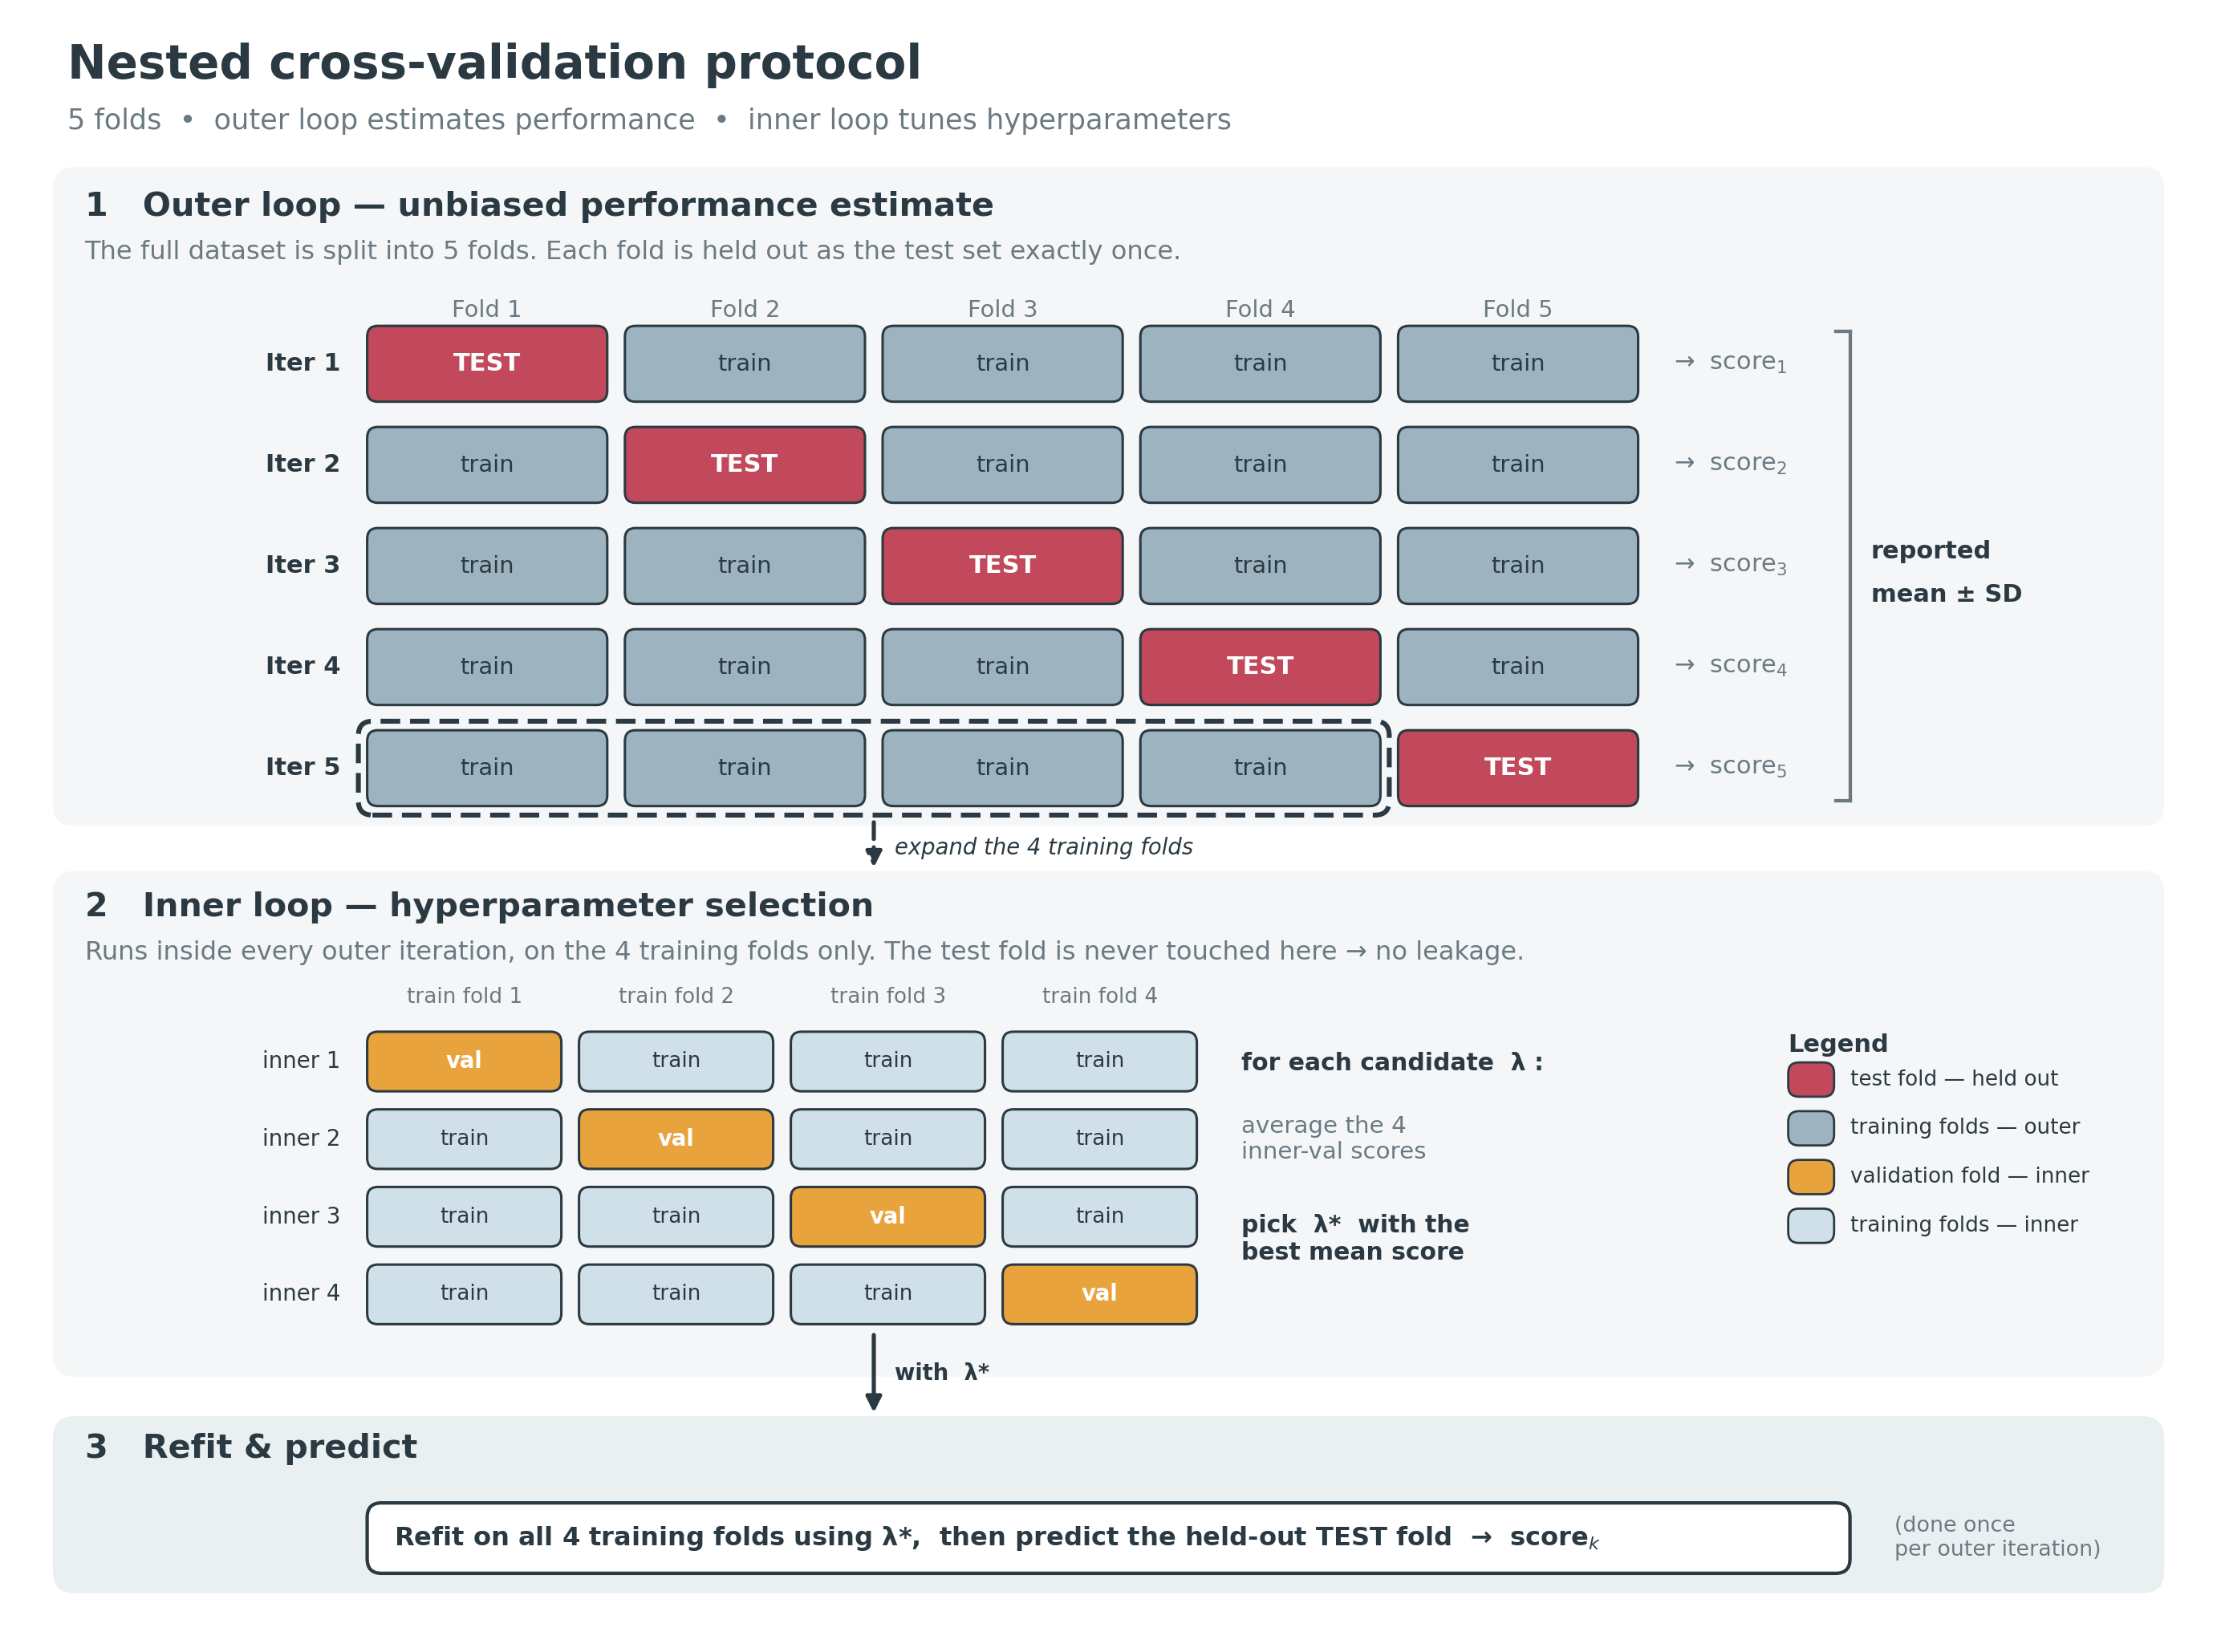
\includegraphics[width=1\textwidth]{figures/nested_cv.png}
\caption{Data partitioning scheme: acquisition-hold groups (60-second holds,
twin-merged across the up- and down-sweep) are partitioned by a single-pass 5-fold
grouped cross-validation. Each fold is scored once by a model tuned and fitted on
the remaining four folds, and the held-out predictions are pooled.}
\label{fig:data_partition}
\end{figure}

\subsection{Model families}
\label{subsec:model_families}

Two regression model families are evaluated across the three sensor configurations,
as summarised in Table~\ref{tab:model_families}. Both are tuned by a group-aware inner cross-validation within each outer training fold---Optuna for LightGBM, \texttt{ElasticNetCV} for Elastic Net---so that fold scores are never contaminated by hyperparameter selection on the held-out data.

\begin{table}[htbp]
\centering
\small
\begin{tabular}{@{} l p{4.5cm} p{8.5cm} @{}}
\toprule
\textbf{Model} & \textbf{Rationale} & \textbf{Hyperparameters \& tuning} \\
\midrule
Elastic Net & $\ell_1$+$\ell_2$ regularised linear model; $\ell_1$ promotes sparsity, $\ell_2$ stabilises correlated features. & $\alpha$ (9 values, $10^{-4}$--$10^{2}$) $\times$ $\ell_1$ ratio (6 values, $0.1$--$1.0$); \texttt{ElasticNetCV}, inner 4-fold grouped. \\[4pt]
LightGBM & Gradient-boosted trees; captures non-linear feature--$\kappa$ mappings and high-order interactions. & Learning rate, num.\ leaves, max.\ depth, min.\ child samples, $\ell_2$ reg.; Bayesian optimisation (Optuna TPE, 20~trials per outer fold). \\
\bottomrule
\end{tabular}
\caption{Regression model families: rationale and hyperparameter tuning strategy.}
\label{tab:model_families}
\end{table}

\subsection{Statistical significance testing}
\label{subsec:sig_tests}

Three cross-sensor comparisons form the study's focal claims: AE vs.\ US, Combined vs.\ AE, and Combined vs.\ US. Each is tested with a group-level modified Diebold--Mariano test~\cite{harvey_testing_1997}. The unit of analysis is the same set of groups used for the regression modelling, so that overly similar segments do not overstate the significance. The squared-error differential $d_i = e_{A,i}^2 - e_{B,i}^2$ is averaged within each holdout group, and the Harvey et al.\ small-sample correction is applied to the resulting $\resNgroups$ group means. The naive segment-level $p$-value is reported alongside each result to make the degree of inflation explicit.

\section{Results}
\label{sec:results}

\subsection{Overall performance}
As Table~\ref{tab:models} shows, all six model--sensor configurations predict $\kappa$ well, with LightGBM ahead of Elastic Net in every one. The size and consistency of this gap indicate a substantially non-linear feature--$\kappa$ mapping, and the close agreement between the per-fold and pooled held-out scores indicates stable generalisation. How much of this accuracy reflects operating-point inference rather than lubrication sensing is the question taken up next.

\begin{table}[H]
\centering
\small
\IfFileExists{tables/table_models_tabular.tex}%
  {% Auto-generated by scripts/07_paper_export.py -- do not edit by hand.
% Values shown as ?? indicate a missing pipeline output; re-run the
% relevant script and then this one.
\begin{tabular}{llcccc}
\toprule
\textbf{Model} & \textbf{Sensors} & \textbf{CV RMSE} & \textbf{HO $R^2$} & \textbf{HO MAE} & \textbf{HO RMSE} \\
\midrule
LightGBM    & Combined & $0.0724 \pm 0.0050$ & \textbf{0.960} & 0.045 & 0.071 \\
LightGBM    & AE       & $0.0784 \pm 0.0041$ & 0.951 & 0.051 & 0.078 \\
LightGBM    & US       & $0.1591 \pm 0.0064$ & 0.805 & 0.101 & 0.155 \\
\midrule
Elastic Net & Combined & $0.1473 \pm 0.0052$ & 0.843 & 0.104 & 0.139 \\
Elastic Net & AE       & $0.1552 \pm 0.0050$ & 0.826 & 0.112 & 0.147 \\
Polynomial  & Combined & $0.1649 \pm 0.0054$ & 0.782 & 0.122 & 0.164 \\
Polynomial  & AE       & $0.1648 \pm 0.0040$ & 0.775 & 0.123 & 0.167 \\
Polynomial  & US       & $0.1988 \pm 0.0045$ & 0.701 & 0.134 & 0.192 \\
Elastic Net & US       & $0.2221 \pm 0.0050$ & 0.628 & 0.155 & 0.214 \\
\bottomrule
\end{tabular}
}%
  {\IfFileExists{../outputs/07_paper_export/table_models_tabular.tex}%
    {% Auto-generated by scripts/07_paper_export.py -- do not edit by hand.
% Values shown as ?? indicate a missing pipeline output; re-run the
% relevant script and then this one.
\begin{tabular}{llcccc}
\toprule
\textbf{Model} & \textbf{Sensors} & \textbf{CV RMSE} & \textbf{HO $R^2$} & \textbf{HO MAE} & \textbf{HO RMSE} \\
\midrule
LightGBM    & Combined & $0.0724 \pm 0.0050$ & \textbf{0.960} & 0.045 & 0.071 \\
LightGBM    & AE       & $0.0784 \pm 0.0041$ & 0.951 & 0.051 & 0.078 \\
LightGBM    & US       & $0.1591 \pm 0.0064$ & 0.805 & 0.101 & 0.155 \\
\midrule
Elastic Net & Combined & $0.1473 \pm 0.0052$ & 0.843 & 0.104 & 0.139 \\
Elastic Net & AE       & $0.1552 \pm 0.0050$ & 0.826 & 0.112 & 0.147 \\
Polynomial  & Combined & $0.1649 \pm 0.0054$ & 0.782 & 0.122 & 0.164 \\
Polynomial  & AE       & $0.1648 \pm 0.0040$ & 0.775 & 0.123 & 0.167 \\
Polynomial  & US       & $0.1988 \pm 0.0045$ & 0.701 & 0.134 & 0.192 \\
Elastic Net & US       & $0.2221 \pm 0.0050$ & 0.628 & 0.155 & 0.214 \\
\bottomrule
\end{tabular}
}%
    {\todo[inline]{Run scripts/07\_paper\_export.py to generate table\_models\_tabular.tex.}}}
\caption{Regression model performance: mean grouped-CV $R^2$ per fold and pooled
held-out $R^2$, MAE, and RMSE. Best pooled $R^2$ in bold.}
\label{tab:models}
\end{table}

\subsection{Operating-point decomposition}
\label{subsec:decomposition}
Because $\kappa$ is a deterministic function of the measured operating point (Eq.~\eqref{eq:kappa}), any $\kappa$-regression performance may in principle be obtained by inferring the operating point acoustically and applying the ISO~281 mapping. To explore this path, a two-stage model is evaluated under the same pooled grouped cross-validation. The features first predict rotational speed and temperature, and the predictions are passed through Eqs.~\eqref{eq:kappa} and \eqref{eq:nu1} to obtain $\kappa$. The feature-to-speed and feature-to-temperature models are LightGBM regressors, trained per fold on the four training folds and scored on the held-out fold, exactly as the direct feature-to-$\kappa$ regression of Table~\ref{tab:models}. Table~\ref{tab:decomposition} compares the two-stage and direct regressions.

\begin{table}[H]
\centering
\small
\begin{tabular}{@{} l c c c c c @{}}
\toprule
\textbf{Channel} & $R^2$ (speed) & $R^2$ (temp.) & $R^2$ ($\kappa$, two-stage) & $R^2$ ($\kappa$, direct) & Residual \\
\midrule
AE       & \resRpmRsqAe   & \resTempRsqAe   & \resTwoStageRsqAe   & \resDirectRsqAe   & \resResidRsqAe \\
US       & \resRpmRsqUs   & \resTempRsqUs   & \resTwoStageRsqUs   & \resDirectRsqUs   & \resResidRsqUs \\
Combined & \resRpmRsqComb & \resTempRsqComb & \resTwoStageRsqComb & \resDirectRsqComb & \resResidRsqComb \\
\bottomrule
\end{tabular}
\caption{Operating-point decomposition (LightGBM, pooled grouped CV): $R^2$ of the
feature-based rotational speed and temperature regressions, the two-stage $\kappa$ estimate
obtained by passing these through the ISO~281 mapping, and the direct $\kappa$
regression. Residual is the direct-minus-two-stage difference.}
\label{tab:decomposition}
\end{table}

Both channels recover the rotational speed and temperature well, with US markedly stronger on temperature, consistent with the conditional correlations shown earlier. For every channel the two-stage $\kappa$ estimate matches the direct regression to within $\approx$0.01~$R^2$, so the direct models perform no better than operating-point inference followed by the ISO~281 mapping. The small positive AE residual is too slight to read as evidence of lubrication-specific sensing. This does not mean the acoustic signals lack lubrication information. Since $\kappa$ is computed from speed and temperature alone, any lubrication effect unrelated to them is absent from $\kappa$, and the decomposition could not detect it even if the signals carried it.

\subsection{Sensor comparison}
\label{subsec:sensor_comparison}
Both channels infer the operating point, so their relative performance turns on which parts of it each captures. Which single channel performs better depends on the model family. Under LightGBM, AE outperforms US while under Elastic Net, the ordering reverses. Both orderings are confirmed by the group-level DM test. A plausible explanation is that the temperature-mediated US structure is closer to linear and is exploited well by Elastic Net, whereas the speed-dependent AE structure is strongly non-linear and requires the tree ensemble. The AE--US gap under LightGBM is in any case small.

\subsection{Sensor fusion}
\label{subsec:sensor_fusion}
The combined feature set outperforms both single channels for both model families, and all four combined-vs-single contrasts are significant under the group-level DM test of Table~\ref{tab:inference}. The absolute $R^2$ gain is
modest, but its consistency across model families and contrasts indicates that
each channel contributes non-redundant information.

\begin{table}[H]
\centering
\small
\begin{tabular}{llrcc}
\toprule
Comparison & Model & $\Delta$RMSE & DM $p$ (group) & DM $p$ (naive) \\
\midrule
AE vs.\ US       & Elastic Net & \resDeltaRmseEnetAeUs   & \resDmGroupEnetAeUs   & \resDmNaiveEnetAeUs \\
                 & LightGBM    & \resDeltaRmseAeUs       & \resDmGroupAeUs       & \resDmNaiveAeUs \\
\midrule
Combined vs.\ AE & Elastic Net & \resDeltaRmseEnetCombAe & \resDmGroupEnetCombAe & \resDmNaiveEnetCombAe \\
                 & LightGBM    & \resDeltaRmseCombAe     & \resDmGroupCombAe     & \resDmNaiveCombAe \\
\midrule
Combined vs.\ US & Elastic Net & \resDeltaRmseEnetCombUs & \resDmGroupEnetCombUs & \resDmNaiveEnetCombUs \\
                 & LightGBM    & \resDeltaRmseCombUs     & \resDmGroupCombUs     & \resDmNaiveCombUs \\
\bottomrule
\end{tabular}
\caption{Cross-sensor significance tests for both model families on the pooled held-out
predictions. $\Delta$RMSE is the point estimate in $\kappa$-units (positive =
first sensor/set better). DM $p$ (group) is the Harvey et al.\ corrected
Diebold--Mariano $p$-value on group-averaged squared-error differentials
($T = \resNgroups$ groups) and DM $p$ (naive) is the uncorrected segment-level
$p$-value.}
\label{tab:inference}
\end{table}
\todo{Shoudl the table not include exact p-values?}

Fig.~\ref{fig:pred_vs_actual} shows predicted vs.\ actual $\kappa$ over the
pooled held-out predictions for both model families and all sensor
configurations, coloured by rotational speed.

\begin{figure}[H]
\centering

\includegraphics[width=\textwidth]{figures/model_pred_vs_actual_holdout.png}
\caption{Predicted vs.\ actual $\kappa$ (pooled held-out predictions) for both model families
and all sensor configurations, coloured by rotational speed. The dashed diagonal indicates perfect
prediction. Residual spread is largest toward the sparsely sampled full-film range
($\kappa > 1$).}
\label{fig:pred_vs_actual}
\end{figure}

Across the grid, predictions track the diagonal most closely for LightGBM whereas Elastic Net compresses the range, over-estimating at low-to-mid $\kappa$-levels and under-estimating at high $\kappa$-levels. Predictions fall into discrete vertical stripes, one per operating
point visited by the staircase. All segments at a given operating point share the same
$\kappa$, so each stripe's vertical scatter is the model's within-operating-point
estimation noise. This scatter is largest toward the sparsely sampled full-film range ($\kappa > 1$) and for the US channel.

\subsection{Clustered SHAP feature importance}
\label{subsec:shap}
The full feature sets contain many strongly correlated features, and SHAP (SHapley Additive exPlanations) importance is split among such near-duplicates, obscuring it. Features are therefore grouped into correlation clusters. Agglomerative hierarchical clustering with average linkage is applied to their pairwise Spearman correlations, and the dendrogram is cut so that features correlated at $|\rho| \geq 0.8$ fall in the same cluster, with each feature assigned to exactly one. Fig.~\ref{fig:shap} reports each cluster's combined importance. The two channels lean on visibly different clusters. AE importance is dominated by a single high-frequency cluster---500~kHz--1~MHz mobility and centre-frequency---well above any other, whereas US importance is led by a baseband amplitude (RMS) cluster together with a few distinct features such as 10--20~kHz mobility. The conditional correlations of Fig.~\ref{fig:marg_cond} tell the same story, with the dominant AE cluster tracking speed and the leading US features leaning towards temperature. The two analyses therefore agree by independent routes.

\begin{figure}[H]
\centering
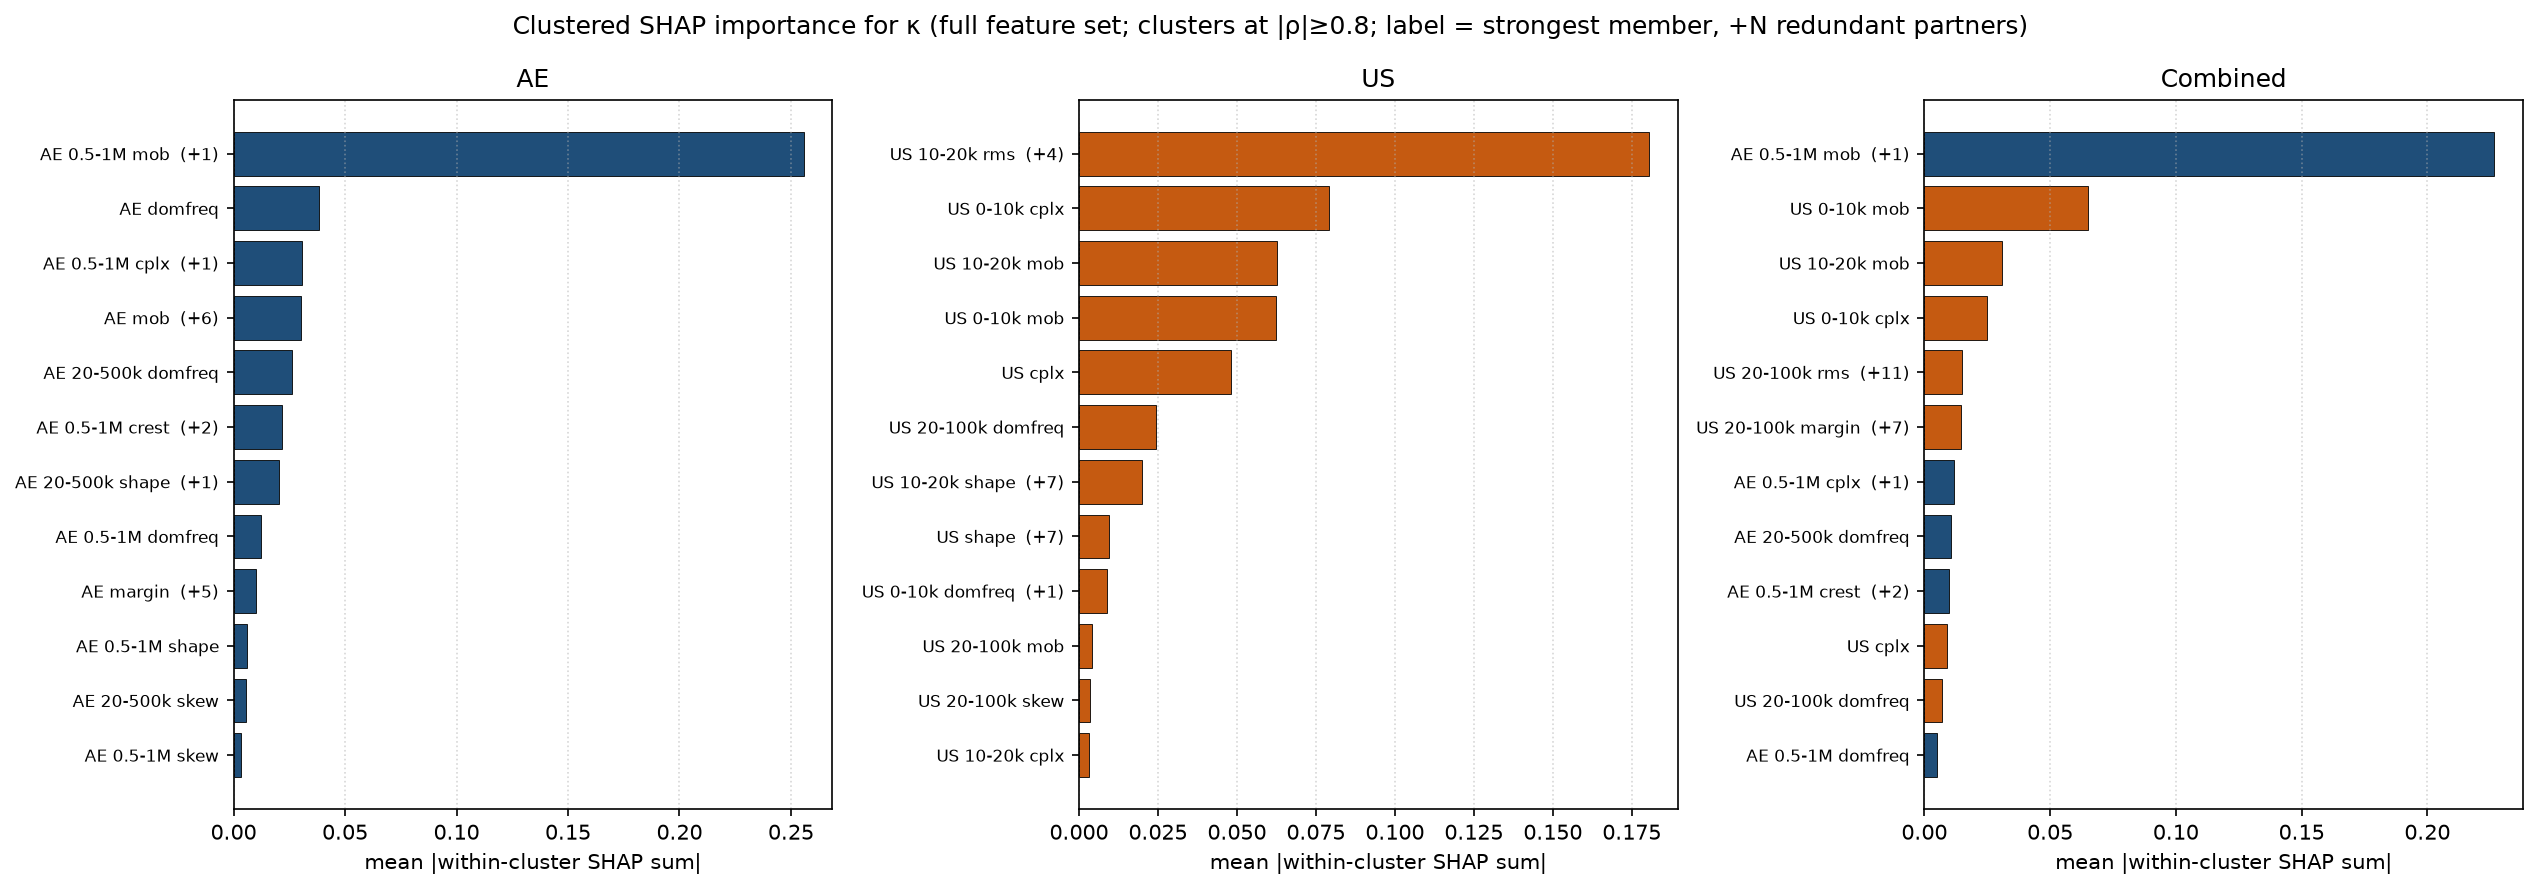
\includegraphics[width=\textwidth]{figures/clustered_shap.png}
\caption{Clustered SHAP importance for $\kappa$ (LightGBM) on the AE, US, and combined
feature sets. Features are grouped into correlation clusters ($|\rho| \geq 0.8$) and each
cluster's summed mean $|\text{SHAP}|$ is plotted, labelled by its strongest member (with
the number of additional correlated members in parentheses); bars are coloured by channel
(blue AE, orange US). AE importance concentrates in a 500~kHz--1~MHz mobility cluster and
US importance in a 10--20~kHz amplitude (RMS) cluster, mirroring the operating-condition
channel separation of Fig.~\ref{fig:marg_cond}. US sub-band labels refer to the probe's
heterodyned audio baseband, not raw acoustic frequencies.}
\label{fig:shap}
\end{figure}
